\documentclass[twoside]{book}

% Packages required by doxygen
\usepackage{fixltx2e}
\usepackage{calc}
\usepackage{doxygen}
\usepackage[export]{adjustbox} % also loads graphicx
\usepackage{graphicx}
\usepackage[utf8]{inputenc}
\usepackage{makeidx}
\usepackage{multicol}
\usepackage{multirow}
\PassOptionsToPackage{warn}{textcomp}
\usepackage{textcomp}
\usepackage[nointegrals]{wasysym}
\usepackage[table]{xcolor}

% Font selection
\usepackage[T1]{fontenc}
\usepackage[scaled=.90]{helvet}
\usepackage{courier}
\usepackage{amssymb}
\usepackage{sectsty}
\renewcommand{\familydefault}{\sfdefault}
\allsectionsfont{%
  \fontseries{bc}\selectfont%
  \color{darkgray}%
}
\renewcommand{\DoxyLabelFont}{%
  \fontseries{bc}\selectfont%
  \color{darkgray}%
}
\newcommand{\+}{\discretionary{\mbox{\scriptsize$\hookleftarrow$}}{}{}}

% Page & text layout
\usepackage{geometry}
\geometry{%
  a4paper,%
  top=2.5cm,%
  bottom=2.5cm,%
  left=2.5cm,%
  right=2.5cm%
}
\tolerance=750
\hfuzz=15pt
\hbadness=750
\setlength{\emergencystretch}{15pt}
\setlength{\parindent}{0cm}
\setlength{\parskip}{3ex plus 2ex minus 2ex}
\makeatletter
\renewcommand{\paragraph}{%
  \@startsection{paragraph}{4}{0ex}{-1.0ex}{1.0ex}{%
    \normalfont\normalsize\bfseries\SS@parafont%
  }%
}
\renewcommand{\subparagraph}{%
  \@startsection{subparagraph}{5}{0ex}{-1.0ex}{1.0ex}{%
    \normalfont\normalsize\bfseries\SS@subparafont%
  }%
}
\makeatother

% Headers & footers
\usepackage{fancyhdr}
\pagestyle{fancyplain}
\fancyhead[LE]{\fancyplain{}{\bfseries\thepage}}
\fancyhead[CE]{\fancyplain{}{}}
\fancyhead[RE]{\fancyplain{}{\bfseries\leftmark}}
\fancyhead[LO]{\fancyplain{}{\bfseries\rightmark}}
\fancyhead[CO]{\fancyplain{}{}}
\fancyhead[RO]{\fancyplain{}{\bfseries\thepage}}
\fancyfoot[LE]{\fancyplain{}{}}
\fancyfoot[CE]{\fancyplain{}{}}
\fancyfoot[RE]{\fancyplain{}{\bfseries\scriptsize Generated by Doxygen }}
\fancyfoot[LO]{\fancyplain{}{\bfseries\scriptsize Generated by Doxygen }}
\fancyfoot[CO]{\fancyplain{}{}}
\fancyfoot[RO]{\fancyplain{}{}}
\renewcommand{\footrulewidth}{0.4pt}
\renewcommand{\chaptermark}[1]{%
  \markboth{#1}{}%
}
\renewcommand{\sectionmark}[1]{%
  \markright{\thesection\ #1}%
}

% Indices & bibliography
\usepackage{natbib}
\usepackage[titles]{tocloft}
\setcounter{tocdepth}{3}
\setcounter{secnumdepth}{5}
\makeindex

% Hyperlinks (required, but should be loaded last)
\usepackage{ifpdf}
\ifpdf
  \usepackage[pdftex,pagebackref=true]{hyperref}
\else
  \usepackage[ps2pdf,pagebackref=true]{hyperref}
\fi
\hypersetup{%
  colorlinks=true,%
  linkcolor=blue,%
  citecolor=blue,%
  unicode%
}

% Custom commands
\newcommand{\clearemptydoublepage}{%
  \newpage{\pagestyle{empty}\cleardoublepage}%
}

\usepackage{caption}
\captionsetup{labelsep=space,justification=centering,font={bf},singlelinecheck=off,skip=4pt,position=top}

%===== C O N T E N T S =====

\begin{document}

% Titlepage & ToC
\hypersetup{pageanchor=false,
             bookmarksnumbered=true,
             pdfencoding=unicode
            }
\pagenumbering{alph}
\begin{titlepage}
\vspace*{7cm}
\begin{center}%
{\Large OO E\+X\+A\+M\+P\+LE }\\
\vspace*{1cm}
{\large Generated by Doxygen 1.8.13}\\
\end{center}
\end{titlepage}
\clearemptydoublepage
\pagenumbering{roman}
\tableofcontents
\clearemptydoublepage
\pagenumbering{arabic}
\hypersetup{pageanchor=true}

%--- Begin generated contents ---
\chapter{Hierarchical Index}
\section{Class Hierarchy}
This inheritance list is sorted roughly, but not completely, alphabetically\+:\begin{DoxyCompactList}
\item \contentsline{section}{Carrinho}{\pageref{class_carrinho}}{}
\item \contentsline{section}{Loja}{\pageref{class_loja}}{}
\item \contentsline{section}{Pessoa}{\pageref{class_pessoa}}{}
\begin{DoxyCompactList}
\item \contentsline{section}{Cliente}{\pageref{class_cliente}}{}
\item \contentsline{section}{Funcionario}{\pageref{class_funcionario}}{}
\end{DoxyCompactList}
\item \contentsline{section}{Produto}{\pageref{class_produto}}{}
\end{DoxyCompactList}

\chapter{Class Index}
\section{Class List}
Here are the classes, structs, unions and interfaces with brief descriptions\+:\begin{DoxyCompactList}
\item\contentsline{section}{\hyperlink{class_carrinho}{Carrinho} }{\pageref{class_carrinho}}{}
\item\contentsline{section}{\hyperlink{class_cliente}{Cliente} }{\pageref{class_cliente}}{}
\item\contentsline{section}{\hyperlink{class_funcionario}{Funcionario} }{\pageref{class_funcionario}}{}
\item\contentsline{section}{\hyperlink{class_loja}{Loja} }{\pageref{class_loja}}{}
\item\contentsline{section}{\hyperlink{class_pessoa}{Pessoa} }{\pageref{class_pessoa}}{}
\item\contentsline{section}{\hyperlink{class_produto}{Produto} }{\pageref{class_produto}}{}
\end{DoxyCompactList}

\chapter{Class Documentation}
\hypertarget{class_carrinho}{}\section{Carrinho Class Reference}
\label{class_carrinho}\index{Carrinho@{Carrinho}}
\subsection*{Public Member Functions}
\begin{DoxyCompactItemize}
\item 
\mbox{\Hypertarget{class_carrinho_a106d07a4475d8aaaf7a9e3cc11a4e30e}\label{class_carrinho_a106d07a4475d8aaaf7a9e3cc11a4e30e}} 
float {\bfseries get\+\_\+valor\+Total} ()
\item 
\mbox{\Hypertarget{class_carrinho_ac375bafe4b800d3433c448677fcf61be}\label{class_carrinho_ac375bafe4b800d3433c448677fcf61be}} 
void {\bfseries set\+\_\+valor\+Total} (float valor\+Total)
\item 
\mbox{\Hypertarget{class_carrinho_aeeb290a496e5345bdf3cf803e5edb43f}\label{class_carrinho_aeeb290a496e5345bdf3cf803e5edb43f}} 
void {\bfseries imprime\+\_\+dados} ()
\end{DoxyCompactItemize}


The documentation for this class was generated from the following files\+:\begin{DoxyCompactItemize}
\item 
inc/carrinho.\+hpp\item 
src/carrinho.\+cpp\end{DoxyCompactItemize}

\hypertarget{class_cliente}{}\section{Cliente Class Reference}
\label{class_cliente}\index{Cliente@{Cliente}}
Inheritance diagram for Cliente\+:\begin{figure}[H]
\begin{center}
\leavevmode
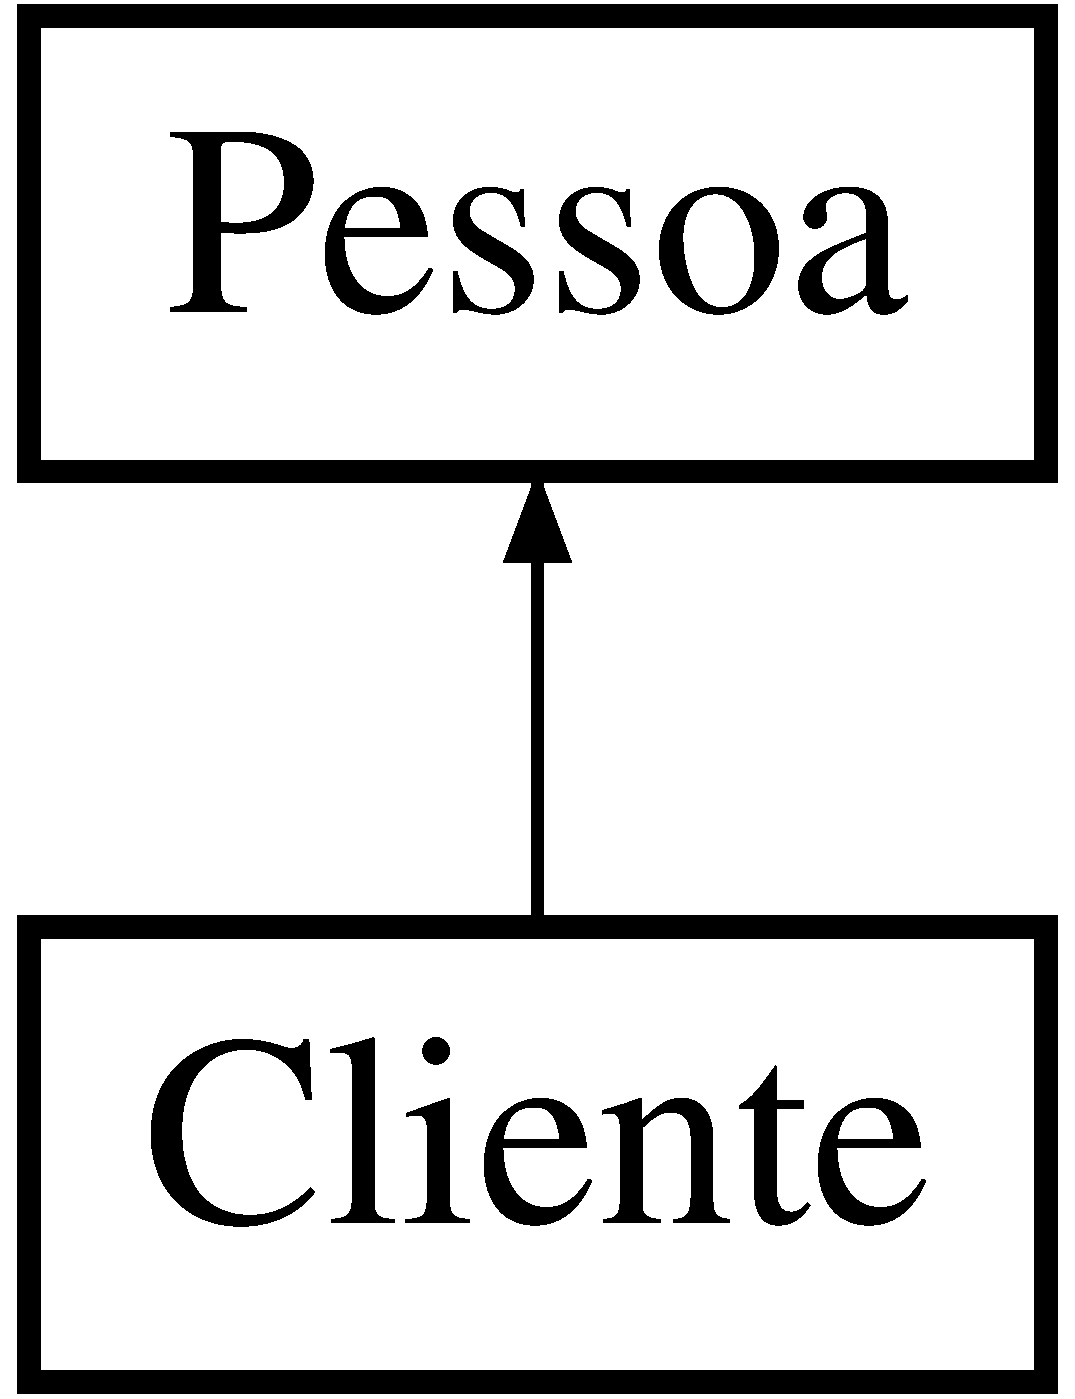
\includegraphics[height=2.000000cm]{class_cliente}
\end{center}
\end{figure}
\subsection*{Public Member Functions}
\begin{DoxyCompactItemize}
\item 
\mbox{\Hypertarget{class_cliente_ae4e880b6374ab92fe40420088b859a89}\label{class_cliente_ae4e880b6374ab92fe40420088b859a89}} 
{\bfseries Cliente} (string nome, string cpf, string email, bool socio)
\item 
\mbox{\Hypertarget{class_cliente_ac19d3bc1957721f87c5605d33d75c020}\label{class_cliente_ac19d3bc1957721f87c5605d33d75c020}} 
bool {\bfseries get\+\_\+socio} ()
\item 
\mbox{\Hypertarget{class_cliente_a13f1249779395a989ef94541ce73435b}\label{class_cliente_a13f1249779395a989ef94541ce73435b}} 
void {\bfseries set\+\_\+socio} (bool socio)
\item 
\mbox{\Hypertarget{class_cliente_a62328e77ee9e9621db1effdb30d44a9f}\label{class_cliente_a62328e77ee9e9621db1effdb30d44a9f}} 
void {\bfseries imprime\+\_\+dados} ()
\end{DoxyCompactItemize}


The documentation for this class was generated from the following files\+:\begin{DoxyCompactItemize}
\item 
inc/cliente.\+hpp\item 
src/cliente.\+cpp\end{DoxyCompactItemize}

\hypertarget{class_funcionario}{}\section{Funcionario Class Reference}
\label{class_funcionario}\index{Funcionario@{Funcionario}}
Inheritance diagram for Funcionario\+:\begin{figure}[H]
\begin{center}
\leavevmode
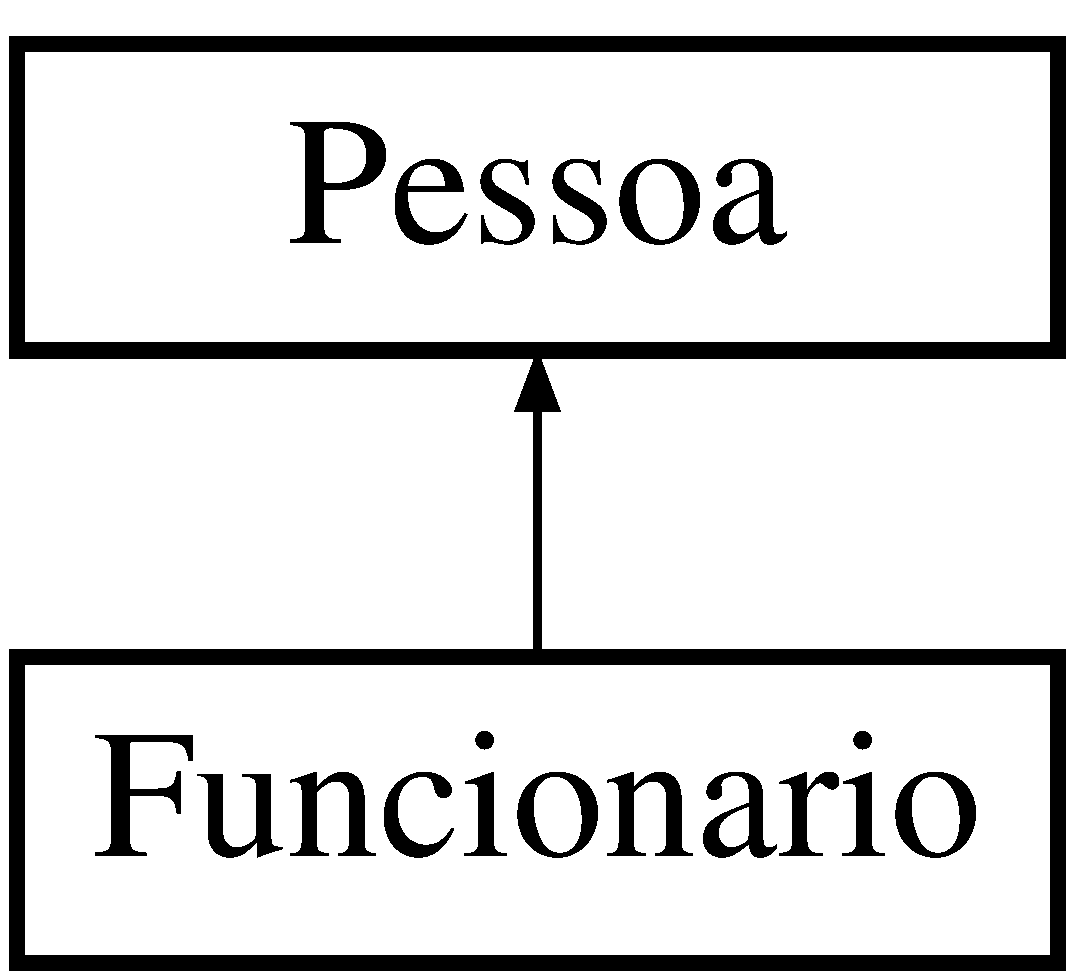
\includegraphics[height=2.000000cm]{class_funcionario}
\end{center}
\end{figure}
\subsection*{Public Member Functions}
\begin{DoxyCompactItemize}
\item 
\mbox{\Hypertarget{class_funcionario_aa86fb3649e63c6039998c6484fe3f61e}\label{class_funcionario_aa86fb3649e63c6039998c6484fe3f61e}} 
{\bfseries Funcionario} (string nome, string cpf, string email, string senha)
\item 
\mbox{\Hypertarget{class_funcionario_a1b39976d01063245c36d3e2532084ef5}\label{class_funcionario_a1b39976d01063245c36d3e2532084ef5}} 
string {\bfseries get\+\_\+senha} ()
\item 
\mbox{\Hypertarget{class_funcionario_a2f6a3b438964dc64418dfe66e0b88c41}\label{class_funcionario_a2f6a3b438964dc64418dfe66e0b88c41}} 
void {\bfseries set\+\_\+senha} (string senha)
\item 
\mbox{\Hypertarget{class_funcionario_a82c56edad048e59b8e64bd194a594287}\label{class_funcionario_a82c56edad048e59b8e64bd194a594287}} 
void {\bfseries imprime\+\_\+dados} ()
\end{DoxyCompactItemize}


The documentation for this class was generated from the following files\+:\begin{DoxyCompactItemize}
\item 
inc/funcionario.\+hpp\item 
src/funcionario.\+cpp\end{DoxyCompactItemize}

\hypertarget{class_loja}{}\section{Loja Class Reference}
\label{class_loja}\index{Loja@{Loja}}
\subsection*{Public Member Functions}
\begin{DoxyCompactItemize}
\item 
\mbox{\Hypertarget{class_loja_a582a978b13027e705591df3d09a249b5}\label{class_loja_a582a978b13027e705591df3d09a249b5}} 
float {\bfseries get\+\_\+valor\+No\+Caixa} ()
\item 
\mbox{\Hypertarget{class_loja_a04aff61cda0d26d86f861ea7956bbe44}\label{class_loja_a04aff61cda0d26d86f861ea7956bbe44}} 
void {\bfseries set\+\_\+valor\+No\+Caixa} (float valor\+No\+Caixa)
\item 
\mbox{\Hypertarget{class_loja_a3342cbf978535dfcdf55d7d604a81424}\label{class_loja_a3342cbf978535dfcdf55d7d604a81424}} 
int {\bfseries confere\+\_\+cliente} ()
\item 
\mbox{\Hypertarget{class_loja_a7399ec3872379f90cbb6a03e7cd6260f}\label{class_loja_a7399ec3872379f90cbb6a03e7cd6260f}} 
void {\bfseries cadastrar\+\_\+cliente} ()
\end{DoxyCompactItemize}
\subsection*{Public Attributes}
\begin{DoxyCompactItemize}
\item 
\mbox{\Hypertarget{class_loja_afdb6d9e9e5001e5eaaf038cc615a3f52}\label{class_loja_afdb6d9e9e5001e5eaaf038cc615a3f52}} 
vector$<$ \hyperlink{class_produto}{Produto} $\ast$ $>$ {\bfseries produtos}
\item 
\mbox{\Hypertarget{class_loja_a24079d9b6184e1b4b7ff127910a78fb7}\label{class_loja_a24079d9b6184e1b4b7ff127910a78fb7}} 
vector$<$ \hyperlink{class_funcionario}{Funcionario} $\ast$ $>$ {\bfseries funcionarios}
\item 
\mbox{\Hypertarget{class_loja_af8abae1471e8367bc9d7b58dbc1a2615}\label{class_loja_af8abae1471e8367bc9d7b58dbc1a2615}} 
vector$<$ \hyperlink{class_cliente}{Cliente} $\ast$ $>$ {\bfseries clientes}
\end{DoxyCompactItemize}


The documentation for this class was generated from the following files\+:\begin{DoxyCompactItemize}
\item 
inc/loja.\+hpp\item 
src/loja.\+cpp\end{DoxyCompactItemize}

\hypertarget{class_pessoa}{}\section{Pessoa Class Reference}
\label{class_pessoa}\index{Pessoa@{Pessoa}}
Inheritance diagram for Pessoa\+:\begin{figure}[H]
\begin{center}
\leavevmode
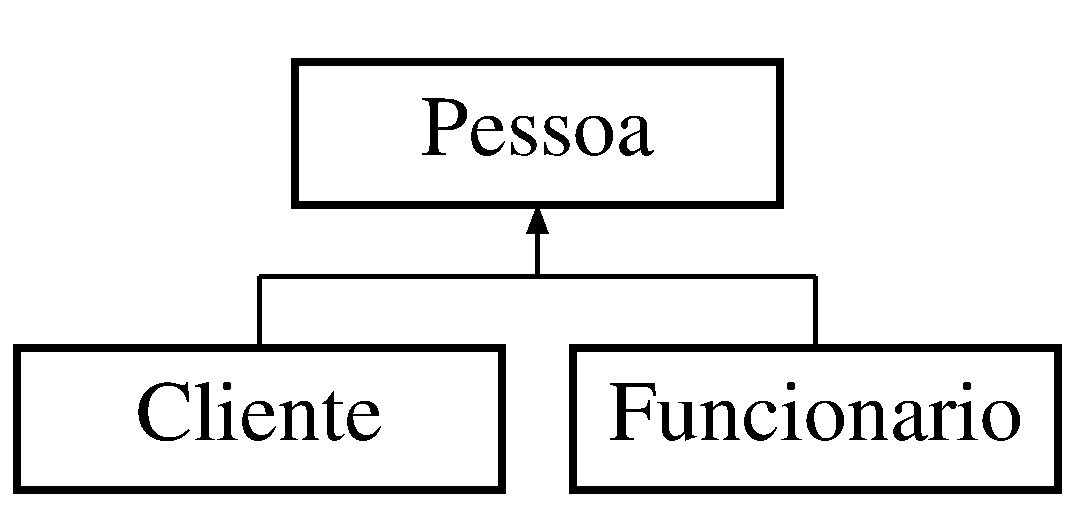
\includegraphics[height=2.000000cm]{class_pessoa}
\end{center}
\end{figure}
\subsection*{Public Member Functions}
\begin{DoxyCompactItemize}
\item 
\mbox{\Hypertarget{class_pessoa_a7bfba3ac538d37d02422346f61bb859d}\label{class_pessoa_a7bfba3ac538d37d02422346f61bb859d}} 
{\bfseries Pessoa} (string nome, string cpf, string email)
\item 
\mbox{\Hypertarget{class_pessoa_a7fc758a1ba17e56d95dfbbc1e65cbedf}\label{class_pessoa_a7fc758a1ba17e56d95dfbbc1e65cbedf}} 
string {\bfseries get\+\_\+nome} ()
\item 
\mbox{\Hypertarget{class_pessoa_afc904106ca6695d07a382a0300f033ba}\label{class_pessoa_afc904106ca6695d07a382a0300f033ba}} 
string {\bfseries get\+\_\+email} ()
\item 
\mbox{\Hypertarget{class_pessoa_a95123b811bca5c1d4c72233b29f227dd}\label{class_pessoa_a95123b811bca5c1d4c72233b29f227dd}} 
string {\bfseries get\+\_\+cpf} ()
\item 
\mbox{\Hypertarget{class_pessoa_ade7bf4832051a8b35b2531632c986b7a}\label{class_pessoa_ade7bf4832051a8b35b2531632c986b7a}} 
void {\bfseries set\+\_\+nome} (string nome)
\item 
\mbox{\Hypertarget{class_pessoa_a829da31a467d19d469925370301c34bd}\label{class_pessoa_a829da31a467d19d469925370301c34bd}} 
void {\bfseries set\+\_\+email} (string email)
\item 
\mbox{\Hypertarget{class_pessoa_ae7fa0ed8427a1674ac87efd327aa2009}\label{class_pessoa_ae7fa0ed8427a1674ac87efd327aa2009}} 
void {\bfseries set\+\_\+cpf} (string cpf)
\item 
\mbox{\Hypertarget{class_pessoa_aa7c97a8759a8813ac14033555dd32ae1}\label{class_pessoa_aa7c97a8759a8813ac14033555dd32ae1}} 
virtual void {\bfseries imprime\+\_\+dados} ()
\end{DoxyCompactItemize}


The documentation for this class was generated from the following files\+:\begin{DoxyCompactItemize}
\item 
inc/pessoa.\+hpp\item 
src/pessoa.\+cpp\end{DoxyCompactItemize}

\hypertarget{class_produto}{}\section{Produto Class Reference}
\label{class_produto}\index{Produto@{Produto}}
\subsection*{Public Member Functions}
\begin{DoxyCompactItemize}
\item 
\mbox{\Hypertarget{class_produto_ac61288fda27dc9801723378e2a8ea621}\label{class_produto_ac61288fda27dc9801723378e2a8ea621}} 
{\bfseries Produto} (string nome, int quantidade, float valor)
\item 
\mbox{\Hypertarget{class_produto_af3226ae7eafdec16f13f266464be7596}\label{class_produto_af3226ae7eafdec16f13f266464be7596}} 
string {\bfseries get\+\_\+nome} ()
\item 
\mbox{\Hypertarget{class_produto_a55230e3937d26a09b2a143a2c2d5173d}\label{class_produto_a55230e3937d26a09b2a143a2c2d5173d}} 
void {\bfseries set\+\_\+nome} (string nome)
\item 
\mbox{\Hypertarget{class_produto_a3fd3e1e0fff93acd3231ec5efd457c7a}\label{class_produto_a3fd3e1e0fff93acd3231ec5efd457c7a}} 
vector$<$ string $>$ {\bfseries get\+\_\+categoria} ()
\item 
\mbox{\Hypertarget{class_produto_a10b0890a8448b51ac46d8c2bc461d3d8}\label{class_produto_a10b0890a8448b51ac46d8c2bc461d3d8}} 
void {\bfseries set\+\_\+categoria} (string categoria)
\item 
\mbox{\Hypertarget{class_produto_a7be9c5aa12a4242a13cac4f624a75167}\label{class_produto_a7be9c5aa12a4242a13cac4f624a75167}} 
int {\bfseries get\+\_\+quantidade} ()
\item 
\mbox{\Hypertarget{class_produto_a7236d29a461f9d28f1dc402b98a8e4af}\label{class_produto_a7236d29a461f9d28f1dc402b98a8e4af}} 
void {\bfseries set\+\_\+quantidade} (int quantidade)
\item 
\mbox{\Hypertarget{class_produto_ad0c2a7a11c09c62ff4988ffa4c220046}\label{class_produto_ad0c2a7a11c09c62ff4988ffa4c220046}} 
float {\bfseries get\+\_\+valor} ()
\item 
\mbox{\Hypertarget{class_produto_af01944f376da523a81130d2a6cbcc661}\label{class_produto_af01944f376da523a81130d2a6cbcc661}} 
void {\bfseries set\+\_\+valor} (float valor)
\item 
\mbox{\Hypertarget{class_produto_a63068fa53c4ad736235e86f4aeaef6af}\label{class_produto_a63068fa53c4ad736235e86f4aeaef6af}} 
bool {\bfseries no\+Estoque} ()
\item 
\mbox{\Hypertarget{class_produto_a46a30f47ffa7f0e98bab6b13ad5e792c}\label{class_produto_a46a30f47ffa7f0e98bab6b13ad5e792c}} 
void {\bfseries imprime\+\_\+dados} ()
\end{DoxyCompactItemize}


The documentation for this class was generated from the following files\+:\begin{DoxyCompactItemize}
\item 
inc/produto.\+hpp\item 
src/produto.\+cpp\end{DoxyCompactItemize}

%--- End generated contents ---

% Index
\backmatter
\newpage
\phantomsection
\clearemptydoublepage
\addcontentsline{toc}{chapter}{Index}
\printindex

\end{document}
